\documentclass{article}
\usepackage{graphicx}
\begin{document}
\begin{center}
  \begin{figure}[htb]
    \centering{
    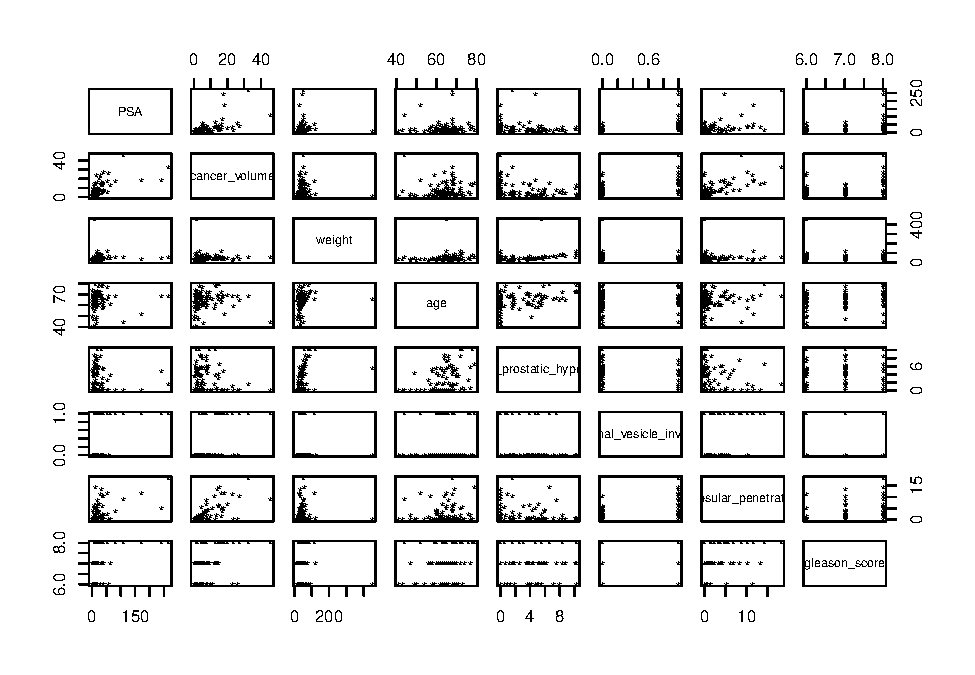
\includegraphics[width=0.8\textwidth]{img/fig1}}
    \caption{scatter plot of quantitative variables}
  \end{figure}

  \begin{figure}
    \centering{
    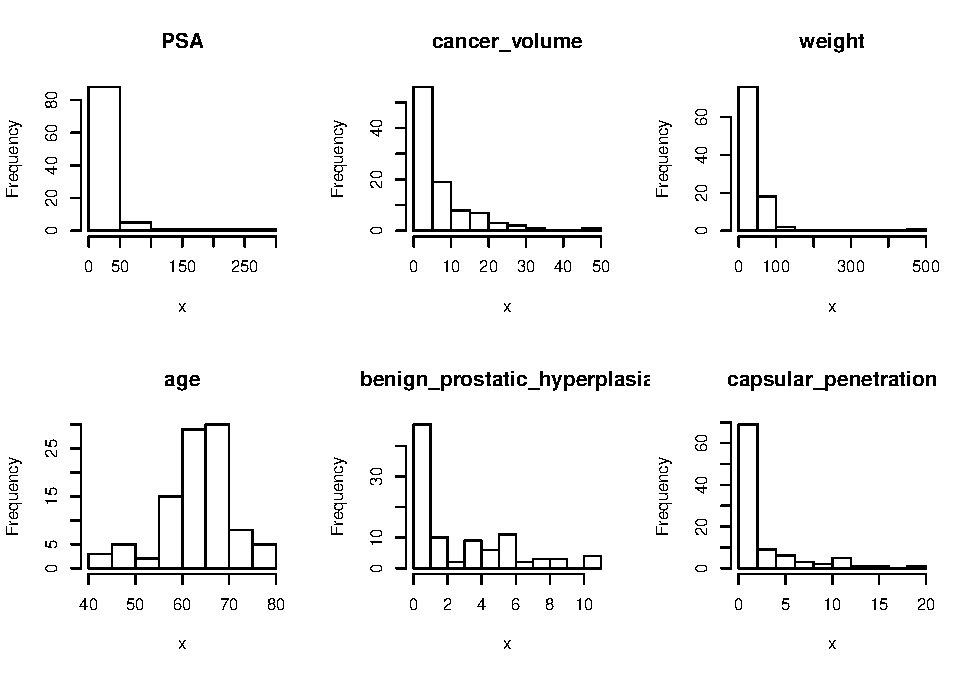
\includegraphics[width=0.8\textwidth]{img/fig2}}
    \caption{histogram of quantitative variables}
  \end{figure}

  \begin{figure}
    \centering{
    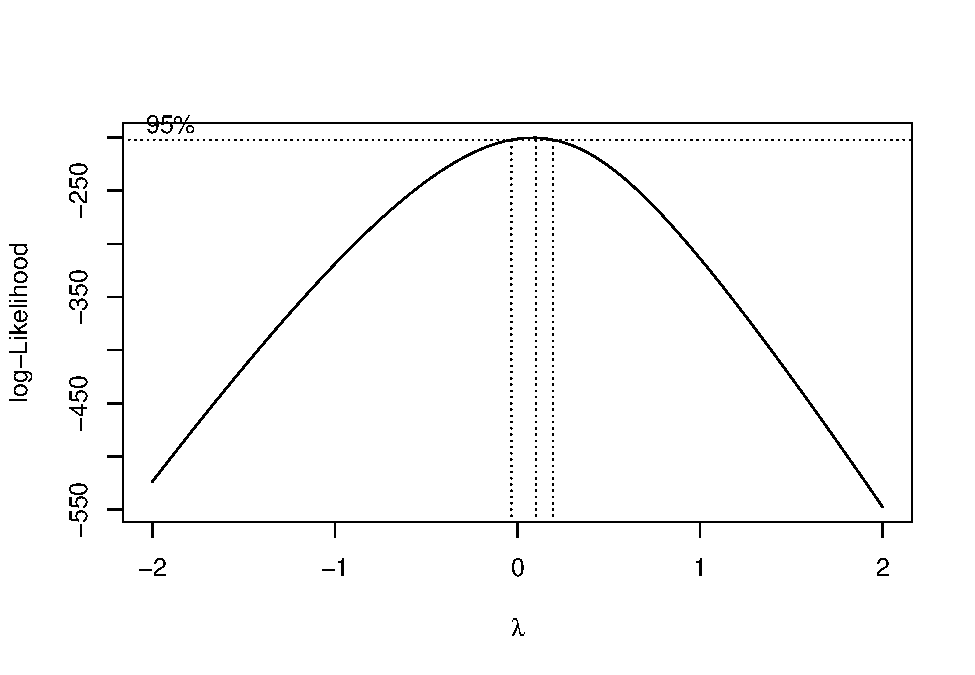
\includegraphics[width=0.8\textwidth]{img/fig3}}
    \caption{Box-Cox plot of PSA}
  \end{figure}

  \begin{figure}
    \centering{
    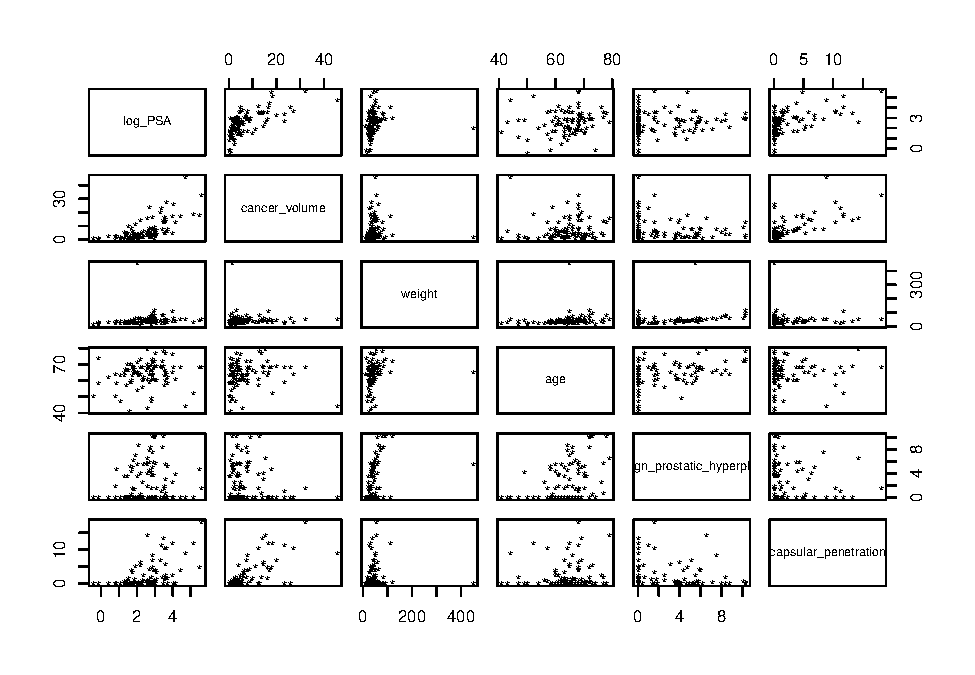
\includegraphics[width=0.8\textwidth]{img/fig4}}
    \caption{scatter plot of transformed quantitative variables}
  \end{figure}

  \begin{figure}
    \centering{
    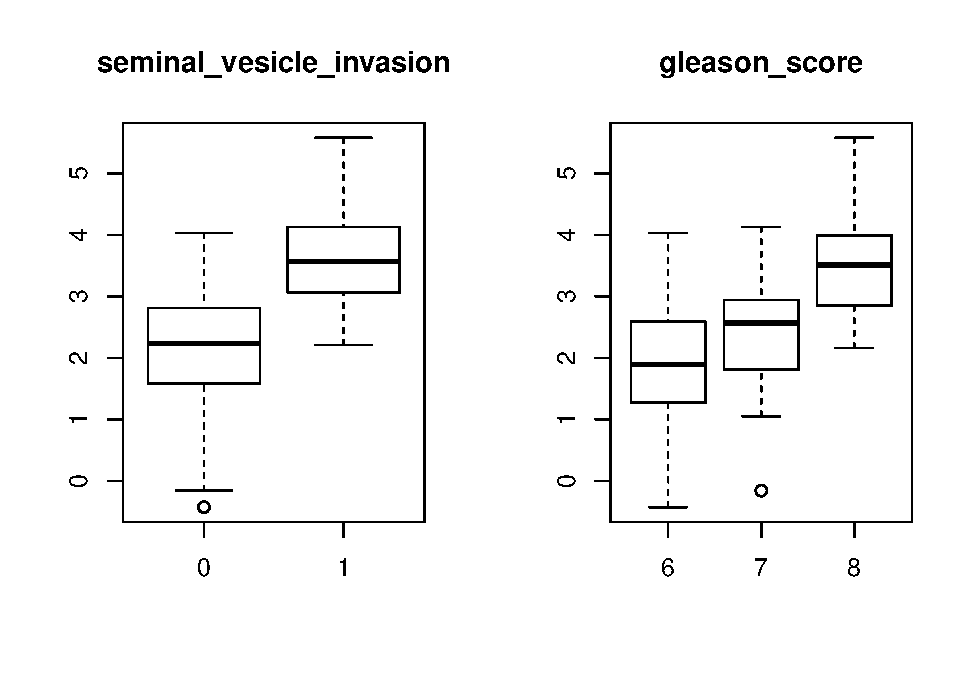
\includegraphics[width=0.8\textwidth]{img/fig6}}
    \caption{side by side boxplot of qualitative variables}
  \end{figure}

  \begin{figure}
    \centering{
    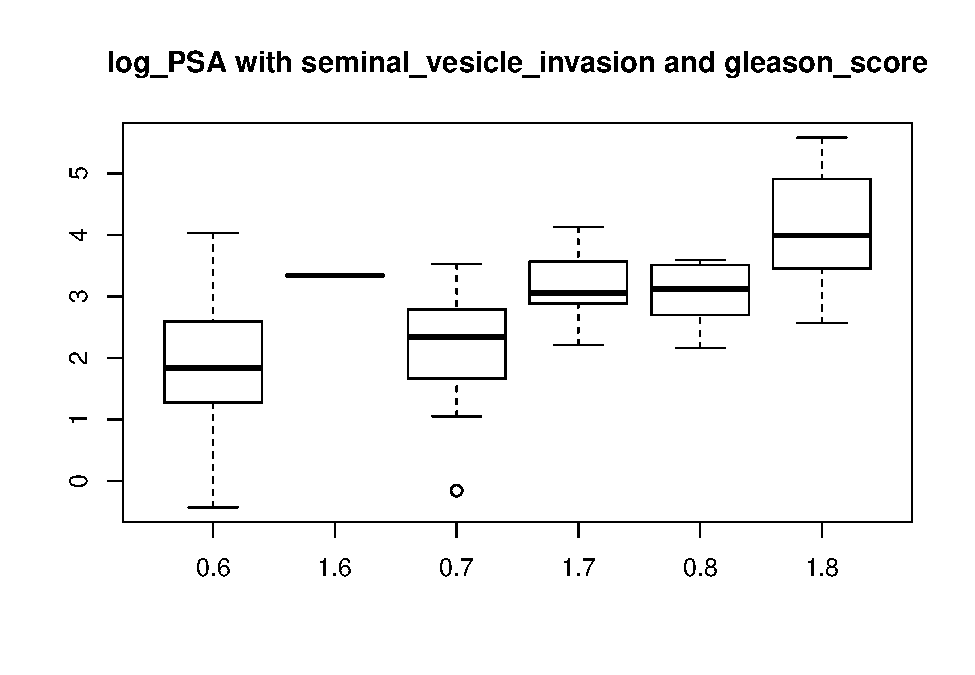
\includegraphics[width=0.8\textwidth]{img/fig7}}
    \caption{side by side boxplot of interaction qualitative variables}
  \end{figure}

  \begin{figure}
    \centering{
    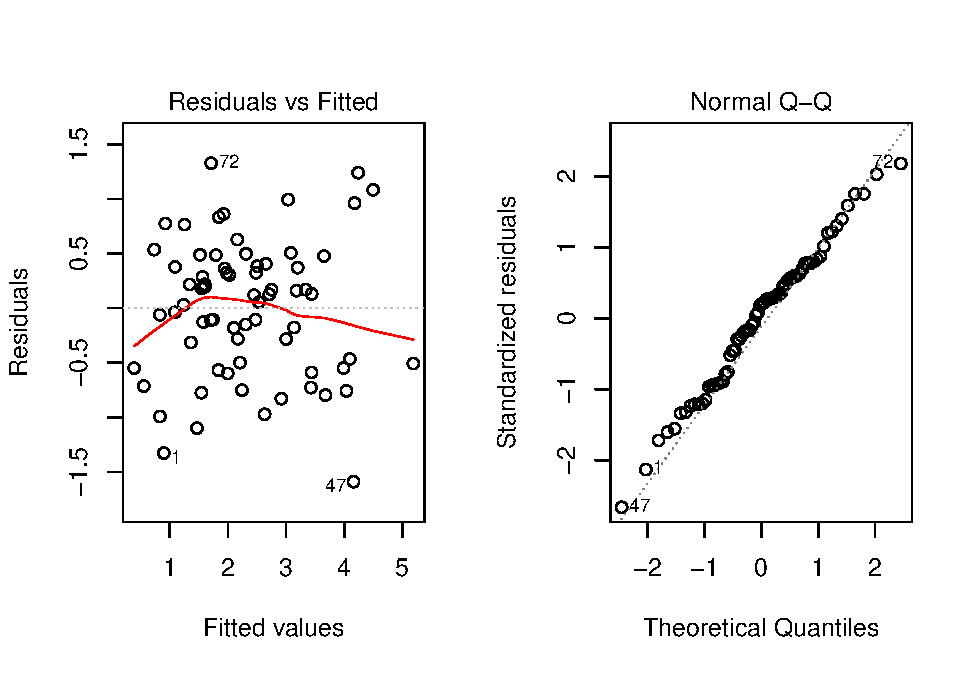
\includegraphics[width=0.65\textwidth]{img/fig8}
    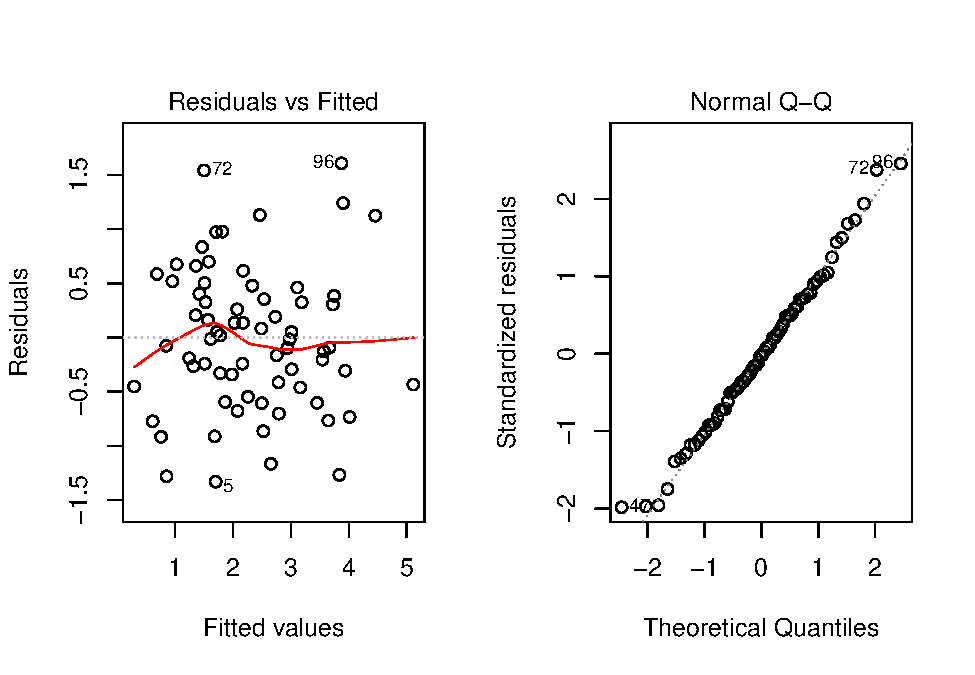
\includegraphics[width=0.65\textwidth]{img/fig9}
    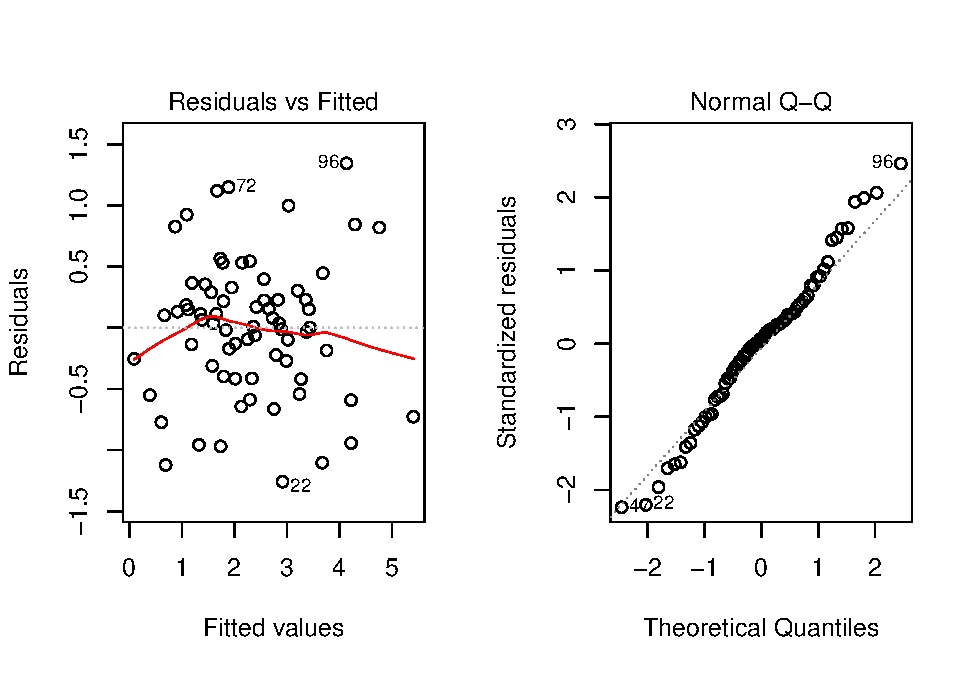
\includegraphics[width=0.65\textwidth]{img/fig10}}
    \caption{residual plots and qqplots of model 1, 2, 3}
  \end{figure}

  \begin{figure}
    \centering{
    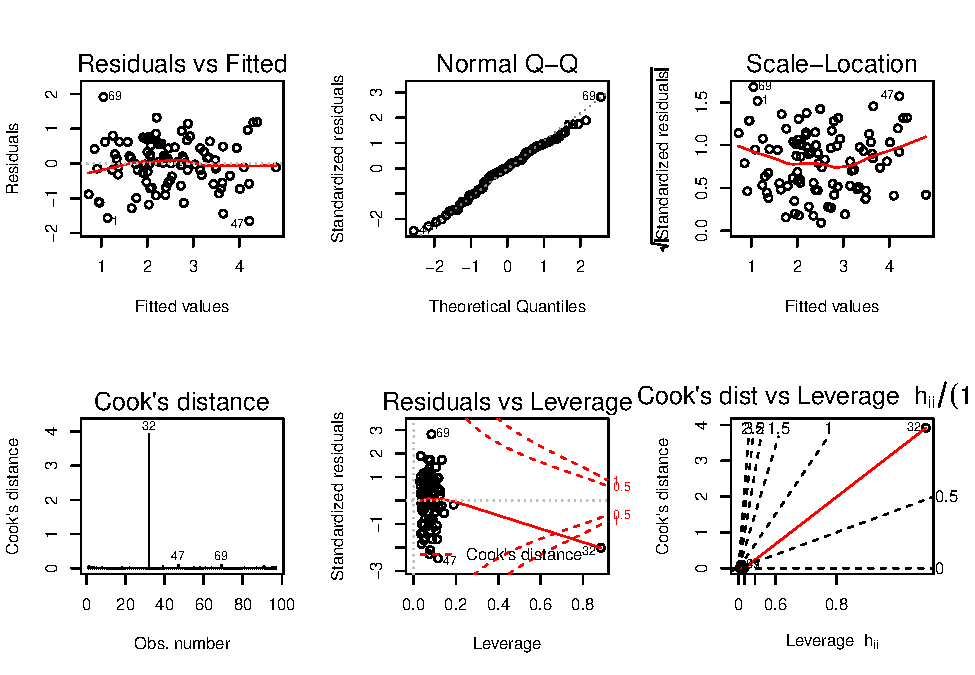
\includegraphics[width=0.8\textwidth]{img/fig11}}
    \caption{model diagnostics of final model}
  \end{figure}

  \begin{figure}
    \centering{
    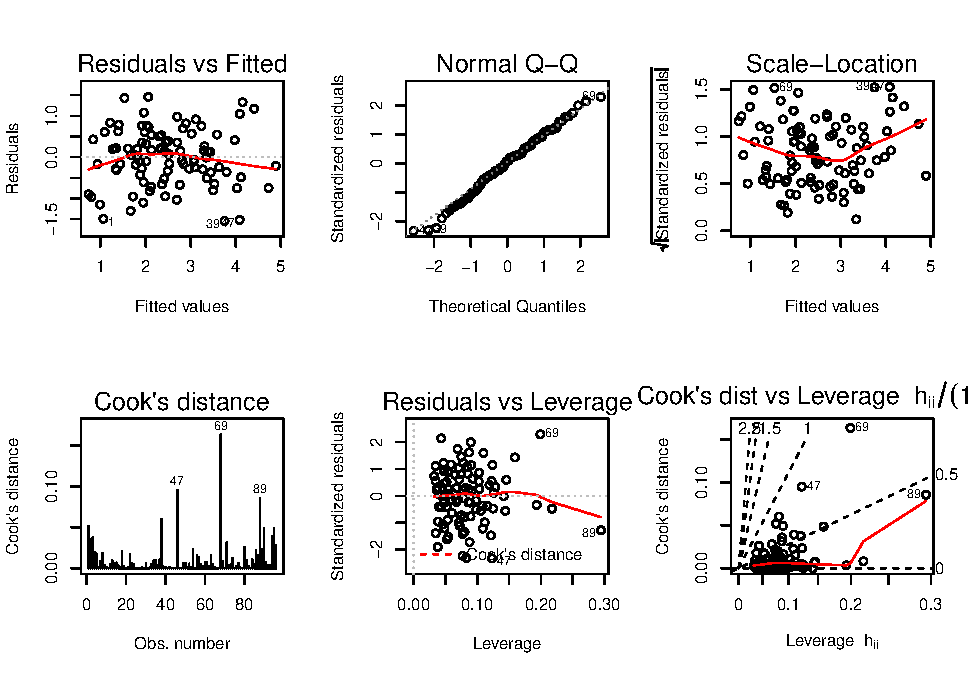
\includegraphics[width=0.8\textwidth]{img/fig12}}
    \caption{model diagnostics of final model (with 32th observation deleted)}
  \end{figure}
\end{center}
\end{document}
